\documentclass{article}
\usepackage[left=3cm,right=3cm,top=2cm,bottom=2cm]{geometry} % page
                                                             % settings
\usepackage{amsmath} % provides many mathematical environments & tools
\usepackage[spanish]{babel}
\usepackage[doument]{ragged2e}

% Images
\usepackage{graphicx}
\usepackage{float}
\usepackage{subfigure} % subfiguras
\usepackage{caption}
\captionsetup[table]{labelformat=empty}
\captionsetup[figure]{labelformat=empty}

% Code
\usepackage{listings}
\usepackage{xcolor}
\definecolor{gray}{rgb}{0.5,0.5,0.5}
\newcommand{\n}[1]{{\color{gray}#1}}
\lstset{numbers=left,numberstyle=\small\color{gray}}

\selectlanguage{spanish}
\usepackage[utf8]{inputenc}
\setlength{\parindent}{0mm}

\usepackage{listings}
\lstset
{ %Formatting for code in appendix
    language=C++,
    basicstyle=\footnotesize,
    numbers=left,
    stepnumber=1,
    showstringspaces=false,
    tabsize=1,
    breaklines=true,
    breakatwhitespace=false,
}


\title{\huge Practica 1: Análisis de Eficiencia de
  Algoritmos\vspace{20mm}}
\author{Patricia Córdoba Hidalgo \\ David
  Cabezas Berrido \\ Emilio Hoyo Medina \\ Inmaculada Marín Carballo}
\date{\vspace{10mm}\today}

\begin{document}
\maketitle

\newpage
\tableofcontents
\newpage

\section{Eficiencia Teórica}

\subsection{Selección:}

En este apartado estudiaremos la eficiencia teórica del algoritmo de ordenación \verb-Selección-, cuyo código en \verb-C++- es el siguiente: 

\begin{lstlisting}
  void seleccion(int T[], int num_elem)
  {
    seleccion_lims(T, 0, num_elem);
  }
  
  static void seleccion_lims(int T[], int inicial, int final)
  {
    int i, j, indice_menor;
    int menor, aux;
    for (i = inicial; i < final - 1; i++) {
      indice_menor = i;
      menor = T[i];
      for (j = i; j < final; j++)
      if (T[j] < menor) {
        indice_menor = j;
        menor = T[j];
      }
      aux = T[i];
      T[i] = T[indice_menor];
      T[indice_menor] = aux;
    };
  }

\end{lstlisting}
La primera función, \verb-seleccion(int T[], int num_elem)-, solo llama a la función \verb-seleccion_lims(int T[],- \\ \verb-int inicial, int final)-, por lo tanto estudiaremos la eficiencia de esta última.

El cuerpo del bucle interno, las líneas 8 y 9, tienen una eficiencia de $O(1)$, luego lo podemos acotar por una constante $a$.
El contenido del bucle \verb-for- interno se ejecuta $final-i$ veces. A su vez, dicho bucle se ejecuta un número de veces igual a $final-1-inicial$. En el bucle externo también se ejecutan otras instrucciones de orden constante, así que llamanos $b$ a la constante que acota la eficiencia de las líneas 11,12,18,19,20.
Así calculamos la eficiencia del algoritmo:

\begin{equation*}
  \sum\limits_{i=inicial}^{final-2}\left(\left(\sum\limits_{j=i}^{final-1}a\right)+b\right) = \sum\limits_{i=inicial}^{final-2}\sum\limits_{j=i}^{final-1}a + \sum\limits_{i=inicial}^{final-2}b
\end{equation*}

Cambiamos la notación, y llamamos $n$ a $final$ y $0$ a $inicial$.

\begin{equation*}
\sum\limits_{i=0}^{n-2}\sum\limits_{j=i}^{n-1}a + \sum\limits_{i=0}^{n-2}b
\end{equation*}

Analizamos las sumatorias por separado:

La primera sumatoria es:

\begin{align*}
  &\sum\limits_{i=0}^{n-2}\sum\limits_{j=i}^{n-1}a
  =\sum\limits_{i=0}^{n-2}a*(n-i)=
  \sum\limits_{i=0}^{n-2}an - \sum\limits_{i=0}^{n-2}ai =
  an(n-1)-a\frac{(n-2)(n-1)}{2} \\
  =&an^2-an-a\frac{n^2-n-2n+2}{2}= 
  an^2-an-\frac{an^2}{2}-\frac{3an}{2}-a=
  \frac{a}{2}n^2-\frac{5a}{2}n-a
\end{align*}

La segunda sumatoria es:
\begin{equation*}
\sum\limits_{i=0}^{n-2}b=b*\sum\limits_{i=0}^{n-2}1=b(n-1)
\end{equation*}

Luego la solución quedaría:

\begin{equation*}
  \sum\limits_{i=inicial}^{final-2}\left(\left(\sum\limits_{j=i}^{final-1}a\right)+b\right) =
  \frac{a}{2}n^2-\frac{5a}{2}n-a + b(n-1) =
  \frac{a}{2}n^2+(b-\frac{5a}{2})n-a-b  
\end{equation*}

En conclusión, la eficiencia del algoritmo de selección es $\frac{a}{2}n^2+(b-\frac{5a}{2})n-a-b$, por lo tanto la eficiencia es $O(n^2)$.


\subsection{Heapsort:}

\begin{lstlisting}
static void heapsort(int T[], int num_elem)
{
  int i;
  for (i = num_elem/2; i >= 0; i--)
    reajustar(T, num_elem, i);
  for (i = num_elem - 1; i >= 1; i--)
    {
      int aux = T[0];
      T[0] = T[i];
      T[i] = aux;
      reajustar(T, i, 0);
    }
}
  

static void reajustar(int T[], int num_elem, int k)
{
  int j;
  int v;
  v = T[k];
  bool esAPO = false;
  while ((k < num_elem/2) && !esAPO)
    {
      j = k + k + 1;
      if ((j < (num_elem - 1)) && (T[j] < T[j+1]))
        j++;
      if (v >= T[j])
        esAPO = true;
      T[k] = T[j];
      k = j;
    }
  T[k] = v;
}
\end{lstlisting}

\begin{flushleft}
  Una llamada a la función con $\text{num\_elem} = n > 0$ elementos
  realiza lo siguiente:

  Primero llama a la función reajustar $\frac{n}{2}+1$ veces. Como
  podemos observar, el bucle de reajustar (línea 22), como máximo, se
  ejecuta $\log_2\frac{n}{2}= \log_2n-1$ ya que el índice k del bucle
  se múltiplica por 2 en cada iteración. El cuerpo del bucle se puede
  acotar por una constante $a$, por lo que la eficiencia de reajustar
  es de $a\log_2n-a$. La función heapsort llama a reajustar en el
  primer bucle $\frac{n}{2}+1$ veces (línea 4), por lo que la
  eficiencia del primer bucle es de $(\dfrac{n}{2}+1)(a\log_2n-a)$ a
  lo sumo. Razonando de forma similar, el segundo bucle (línea 6), que
  se ejecuta $n-1$ veces, tiene una eficiencia de
  $a(n-1)(\log_2(n)-1)+b(n-1)$, acotando el cuerpo del bucle (líneas
  8, 9, 10) por una constante $b$. La eficiencia total es el máximo de
  los dos, que en cualquier caso es $O(nlog n)$.
\end{flushleft}

\subsection{Floyd:}

En este apartado estudiaremos la eficiencia teórica del algoritmo de Floyd, cuyo código en \verb-C++- es el siguiente: 

\begin{lstlisting}
  void Floyd(int **M, int dim)
  {
    for (int k = 0; k < dim; k++)
    for (int i = 0; i < dim;i++)
    for (int j = 0; j < dim;j++)
    {
      int sum = M[i][k] + M[k][j];    	
      M[i][j] = (M[i][j] > sum) ? sum : M[i][j];
    }
  }
\end{lstlisting}

Podemos observar que dentro del bucle interno, en la línea 7 y 8, las operaciones que de realizan son todas $O(1)$, luego el valor de la eficiencia es constante. Llamemos a dicha constante $a$.
Estas operaciones se realizan n veces en cada uno de los bucles, siendo n la dimensión del grafo, correspondiente con la variable dim. La eficiencia de dicho algoritmo se calcula:

$$\sum\limits_{k=0}^n\sum\limits_{i=o}^n\sum\limits_{j=0}^na=an^3$$

Luego la eficiencia del algoritmo de Floyd es de $o(n^3)$.

\subsection{Hanoi:}
En este apartado estudiaremos la eficiencia teórica del algoritmo de Hanoi, cuyo código en \verb-C++- es el siguiente: 

\begin{lstlisting}
void hanoi (int M, int i, int j)
{
  if (M > 0)
  {
      hanoi(M-1, i, 6-i-j);
      cout << i << " -> " << j << endl;
      hanoi (M-1, 6-i-j, j);
  }
}
\end{lstlisting}

\begin{flushleft}
  Una llamada a la función con $M > 0$ elementos realiza lo siguiente:
  \begin{itemize}
    \item[\textbf{Línea 5:}] Una llamada a esa misma función con $M-1$ elementos, para desplazar
      los $M-1$ discos superiores a otra varilla ($T(M-1)$).

    \item[\textbf{Línea 6:}] Un movimiento para desplazar el disco inferior, de
      eficiencia constante (podemos acotarla por $a$).

    \item[\textbf{Línea 7:}] Una llamada a esa misma función con $M-1$ elementos, para colocar
      los $M-1$ discos superiores de nuevo sobre el disco grande ($T(M-1)$).
  \end{itemize}

  De aquí podemos deducir que la eficiencia del algoritmo cumple la
  siguiente ecuación de recurrencia:
  \[T(M) = T(M-1) + a + T(M-1) = 2T(M-1)+a\]

  Hallamos la ecuación característica:
  \[(x-2)(x-1) = 0\]

  Por tanto se tendrá:
  \[T(M) = c_12^M+c_2\]

  Para algunas constantes $c_1, c_2$, por lo que deducimos que este
  algoritmo es del orden de eficiencia $O(2^n)$ donde $n$ es el número
  de discos.
\end{flushleft}

\section{Eficiencia Empírica:}
\subsection{Algoritmos de Ordenación:}

\begin{figure}[H]
\hspace{-20mm}
\mbox{
\subfigure[Burbuja]{
\begin{tabular}{|c|c|c|c|c|}
\hline
\multicolumn{1}{|c|}{$\textbf{n}$}& 
\textbf{Patricia}& 
\textbf{David}& 
\textbf{Inma}&
\textbf{Emilio}\\ \hline
    1000       & 0.005976 & 0.004416  & 0.003965 & 0.010925 \\
    2000       & 0.015512 & 0.009701  & 0.009249 & 0.027964 \\
    3000       & 0.034809 & 0.021534    & 0.019963 & 0.022135 \\
    4000       & 0.067088 & 0.033732  & 0.036335 & 0.034394 \\
    5000       & 0.108551 & 0.052993  & 0.059549 & 0.056704  \\
    6000       & 0.160577 & 0.0785  & 0.084189 & 0.085118 \\
    7000       & 0.227454 & 0.116606  & 0.118284 & 0.120264 \\
    8000       & 0.308013 & 0.157316  & 0.157555 & 0.162368  \\
    9000       & 0.396967 & 0.198552  & 0.206014 & 0.211109\\
    10000      & 0.504398 & 0.244325  & 0.256693 & 0.266616\\
    11000      & 0.611098 & 0.297715  & 0.31667  & 0.327861\\
    12000      & 0.74526  & 0.355768  & 0.378848 & 0.392673 \\
    13000      & 0.883979 & 0.421353  & 0.451885 & 0.473604 \\
    14000      & 1.02945  & 0.490008  & 0.533033 & 0.551242\\
    15000      & 1.18258  & 0.565647  & 0.61236  & 0.637034\\
    16000      & 1.36519  & 0.648838  & 0.702706 & 0.729671\\
    17000      & 1.54529  & 0.734952  & 0.79395  & 0.835558\\
    18000      & 1.73832  & 0.825036   & 0.901772 & 0.934124\\
    19000      & 1.94908  & 0.925171   & 1.01773  & 1.04908\\
    20000      & 2.16786  & 1.02862  & 1.13979  & 1.17735\\
    21000      & 2.3977   & 1.13798  & 1.24116  & 1.29866 \\
    22000      & 2.64076  & 1.2548   & 1.36741  & 1.42678 \\
    23000      & 2.89207  & 1.37147    & 1.50074  & 1.57506\\
    24000      & 3.16667  & 1.53636   & 1.6442   & 1.71986\\
    25000      & 3.4333   & 1.67428   & 1.78154  & 1.8829 \\ \hline    
  \end{tabular}

}
\qquad
\subfigure[Inserción]{
\begin{tabular}{|c|c|c|c|c|}
\hline
\multicolumn{1}{|c|}{$\textbf{n}$}& 
\textbf{Patricia}&
\textbf{David}&
\textbf{Inma}&
\textbf{Emilio}\\\hline
    1000       & 0.004482  & 0.001242 & 0.002591 & 0.007191 \\
    2000       & 0.012767  & 0.005147 & 0.005385 & 0.016591 \\
    3000       & 0.0225    & 0.012807 & 0.011217 & 0.013373 \\
    4000       & 0.034097  & 0.020767 & 0.01875  & 0.018308 \\
    5000       & 0.051186  & 0.024215 & 0.027998 & 0.027142 \\
    6000       & 0.074354  & 0.034137 & 0.041611 & 0.038888 \\
    7000       & 0.102134  & 0.046124 & 0.053026 & 0.050754 \\
    8000       & 0.131137  & 0.059695 & 0.067336 & 0.070544 \\
    9000       & 0.165877  & 0.074662 & 0.083171 & 0.085773 \\
    10000      & 0.204467  & 0.092759 & 0.104916 & 0.105822 \\
    11000      & 0.246159  & 0.11217  & 0.12479  & 0.129135 \\
    12000      & 0.293801  & 0.13501  & 0.14993  & 0.153725 \\
    13000      & 0.341684  & 0.157762 & 0.176463 & 0.178786 \\
    14000      & 0.395323  & 0.182619 & 0.200255 & 0.206976 \\
    15000      & 0.464424  & 0.208906 & 0.230315 & 0.236186 \\
    16000      & 0.521728  & 0.239027 & 0.266914 & 0.270458 \\
    17000      & 0.586975  & 0.266649 & 0.29109  & 0.307249 \\
    18000      & 0.66804   & 0.301845 & 0.326361 & 0.34197 \\
    19000      & 0.73381   & 0.334605 & 0.366154 & 0.380368 \\
    20000      & 0.866409  & 0.368961 & 0.40182  & 0.423442 \\
    21000      & 0.992073  & 0.407094 & 0.442191 & 0.462617 \\
    22000      & 1.00903   & 0.448405 & 0.486678 & 0.508855 \\
    23000      & 1.0937    & 0.491561 & 0.53288  & 0.55769 \\
    24000      & 1.18201   & 0.537183 & 0.58414  & 0.60885 \\
    25000      & 1.29502   & 0.586868 & 0.630364 & 0.666086 \\ \hline
    
\end{tabular}
}
}
\end{figure}

\begin{figure}[H]
\hspace{-20mm}
\mbox{
\subfigure[Selección]{
\begin{tabular}{|c|c|c|c|c|}
\hline
\multicolumn{1}{|c|}{$\textbf{n}$}& 
\textbf{Patricia}& 
\textbf{David}& 
\textbf{Inma}&
\textbf{Emilio}\\ \hline

    1000       & 0.00262757 & 0.00132932 & 0.00142768 & 0.00146965 \\
    2000       & 0.00988708 & 0.00472456 & 0.00527518 & 0.00540337 \\
    3000       & 0.022101   & 0.010695 & 0.012787 & 0.012246 \\
    4000       & 0.03958    & 0.018866 & 0.022011 & 0.021857 \\
    5000       & 0.061487   & 0.029365 & 0.034569 & 0.033978 \\
    6000       & 0.087545   & 0.042309 & 0.048853 & 0.048972 \\
    7000       & 0.119015   & 0.057128 & 0.065342 & 0.065604 \\
    8000       & 0.15565    & 0.074368 & 0.086007 & 0.085406  \\
    9000       & 0.198281   & 0.093737 & 0.107436 & 0.108106  \\
    10000      & 0.243808   & 0.115629 & 0.134774 &  0.133152 \\
    11000      & 0.295881   & 0.140806 & 0.158507 &  0.160211 \\
    12000      & 0.351218   & 0.166908 & 0.187981 &  0.189744 \\
    13000      & 0.41296    & 0.195358 & 0.219172 &  0.223452 \\
    14000      & 0.477647   & 0.226432 & 0.26315  &  0.258524 \\
    15000      & 0.558161   & 0.260561 & 0.290349 &  0.295088 \\
    16000      & 0.628378   & 0.294718 & 0.331224 &  0.33748  \\
    17000      & 0.706317   & 0.334074 & 0.372539 &  0.37864  \\
    18000      & 0.798014   & 0.373655 & 0.415924 &  0.426695 \\
    19000      & 0.883091   & 0.416012 & 0.463406 &  0.476603 \\
    20000      & 0.978653   & 0.461119 & 0.513847 &  0.528334 \\
    21000      & 1.08933    & 0.508379 & 0.566082 &  0.582423 \\
    22000      & 1.18757    & 0.558152 & 0.620469 &  0.646925 \\
    23000      & 1.29516    & 0.608983 & 0.676672 &  0.69357  \\
    24000      & 1.41024    & 0.662848 & 0.736138 &  0.752397 \\
    25000      & 1.53129    & 0.719359 & 0.8008   &  0.820279 \\ \hline
  
  \end{tabular}

}
\qquad
\subfigure[Quicksort]{
\begin{tabular}{|c|c|c|c|c|}
\hline
\multicolumn{1}{|c|}{$\textbf{n}$}& 
\textbf{Patricia}&
\textbf{David}&
\textbf{Inma}&
\textbf{Emilio}\\\hline

    1000       & 0.000162 & 0.000349 & 0.000308  & 0.000162  \\
    2000       & 0.000741 & 0.000921 & 0.000667  & 0.000382  \\
    3000       & 0.000698 & 0.000349 & 0.001053  & 0.000592  \\
    4000       & 0.001012 & 0.000482 & 0.001426  & 0.000741  \\
    5000       & 0.001266 & 0.000606 & 0.001791  & 0.000946  \\
    6000       & 0.001497 & 0.000764 & 0.002248  & 0.001166  \\
    7000       & 0.001639 & 0.00101  & 0.00261   & 0.001426  \\
    8000       & 0.00178  & 0.001136 & 0.003053  & 0.00171   \\
    9000       & 0.00204  & 0.001303 & 0.002372  & 0.001534  \\
    10000      & 0.00218  & 0.001499 &  0.002681 &  0.001609 \\
    11000      & 0.002356 & 0.001428 &  0.002944 &  0.001588 \\
    12000      & 0.002482 & 0.001595 &  0.002475 &  0.001574 \\
    13000      & 0.002704 & 0.001735 &  0.002209 &  0.001717 \\
    14000      & 0.002886 & 0.001877 &  0.002375 &  0.001947 \\
    15000      & 0.003156 & 0.002125 &  0.002569 &  0.002018 \\
    16000      & 0.003379 & 0.002158 &  0.002763 &  0.002148 \\
    17000      & 0.003766 & 0.002309 &  0.002951 &  0.002267 \\
    18000      & 0.00384  & 0.002161 &  0.00316  &  0.002465 \\
    19000      & 0.004111 & 0.002223 &  0.003129 &  0.00254  \\
    20000      & 0.004328 & 0.002341 &  0.002994 &  0.00266  \\
    21000      & 0.004988 & 0.002306 &  0.003123 &  0.00282  \\
    22000      & 0.006151 & 0.002397 &  0.003315 &  0.002993 \\
    23000      & 0.005015 & 0.002619 &  0.003488 &  0.003073 \\
    24000      & 0.00555  & 0.002889 &  0.003624 &  0.003226 \\
    25000      & 0.005491 & 0.002906 &  0.003809 &  0.003372 \\ \hline
    
\end{tabular}
}
}
\end{figure}


\begin{figure}[H]
\hspace{-20mm}
\mbox{
\subfigure[Mergesort]{
\begin{tabular}{|c|c|c|c|c|}
\hline
\multicolumn{1}{|c|}{$\textbf{n}$}&
\textbf{Patricia}&
\textbf{David}&
\textbf{Inma}&
\textbf{Emilio}\\ \hline
1000 & 0.00022471  & 0.000111503 & 0.000123555 & 0.000124611 \\
2000 & 0.000509159 & 0.000235082 & 0.00026411  & 0.000270196 \\
3000 & 0.000956685 & 0.000433307 & 0.000503566 & 0.000505818 \\
4000 & 0.00109254  & 0.000507335 & 0.000601595 & 0.000589294 \\
5000 & 0.00154249  & 0.000711784 & 0.000785834 & 0.000820999 \\
6000 & 0.00205731  & 0.000933769 & 0.00105483  & 0.00107757 \\
7000 & 0.00196719  & 0.000906519 & 0.00100817  & 0.00104934 \\
8000 & 0.00242298  & 0.00109287  & 0.00122049  & 0.00125782 \\
9000 & 0.00287169  & 0.0012998   & 0.00144209  & 0.00148825 \\
10000 & 0.00329314 & 0.00151355  & 0.00167401  & 0.00174292 \\
11000 & 0.003829   & 0.001805    & 0.001938    & 0.002003 \\
12000 & 0.004369   & 0.002079    & 0.002407    & 0.00233 \\
13000 & 0.003989   & 0.001935    & 0.001979    & 0.002099 \\
14000 & 0.004278   & 0.001973    & 0.002609    & 0.002372 \\
15000 & 0.004743   & 0.002167    & 0.002434    & 0.002542 \\
16000 & 0.005097   & 0.002389    & 0.002785    & 0.002793 \\
17000 & 0.005548   & 0.002663    & 0.003253    & 0.003046 \\
18000 & 0.006182   & 0.002867    & 0.003561    & 0.003572 \\
19000 & 0.006647   & 0.003284    & 0.003797    & 0.003633 \\
20000 & 0.007024   & 0.003441    & 0.004108    & 0.003852 \\
21000 & 0.007573   & 0.003775    & 0.004382    & 0.004168 \\
22000 & 0.00817    & 0.004023    & 0.004189    & 0.00441 \\
23000 & 0.011889   & 0.004289    & 0.005035    & 0.005344 \\
24000 & 0.009352   & 0.004311    & 0.005164    & 0.004963 \\
25000 & 0.011288   & 0.004956    & 0.005336    & 0.005261 \\ \hline
\end{tabular}
}
\qquad
\subfigure[Heapsort]{
\begin{tabular}{|c|c|c|c|c|}
\hline
\multicolumn{1}{|c|}{$\textbf{n}$}& 
\textbf{Patricia}&
\textbf{David}&
\textbf{Inma}&
\textbf{Emilio}\\\hline
      1000    & 0.000329  & 0.000452&0.000449&0.000209  \\
      2000    & 0.000614  & 0.001106&0.000972&0.000455  \\
      3000    & 0.000766  & 0.001416&0.001369&0.000932   \\
      4000    & 0.001059  & 0.000682&0.000645&0.001269    \\
      5000    & 0.001352  & 0.000806&0.000932&0.001851    \\
      6000    & 0.001559  & 0.000984&0.001149&0.001936    \\
      7000    & 0.001842  & 0.001154&0.001352&0.002254   \\
      8000    & 0.002287  & 0.001349&0.001521&0.002593    \\ 
      9000    & 0.002468  & 0.001527&0.001537&0.00294     \\
      10000   & 0.002789  & 0.001716&0.001724&0.002498    \\
      11000   & 0.003093  & 0.002097&0.001902&0.002389    \\
      12000   & 0.003383  & 0.002104&0.002096&0.002264   \\
      13000   & 0.003739  & 0.002302&0.002294&0.002349    \\
      14000   & 0.004009  & 0.002499&0.002485&0.002684    \\
      15000   & 0.004366  & 0.002801&0.002702&0.00279     \\
      16000   & 0.004838  & 0.002912&0.002902&0.002829   \\
      17000   & 0.005016  & 0.003118&0.003126&0.003008   \\
      18000   & 0.005356  & 0.003316&0.003332&0.003238    \\
      19000   & 0.005662  & 0.00357 &0.00351 &0.003383     \\
      20000   & 0.00617   & 0.003735&0.003718&0.003589     \\
      21000   & 0.006625  & 0.003925&0.003913&0.003998      \\
      22000   & 0.006772  & 0.003771&0.004123&0.004014    \\
      23000   & 0.007206  & 0.003569&0.004332&0.004179    \\
      24000   & 0.007361  & 0.003566&0.004546&0.005269    \\
      25000   & 0.007712  & 0.003972&0.004751&0.00508     \\ \hline
\end{tabular}
}
}
\end{figure}


\subsection{Floyd y Hanoi:}

\begin{figure}[H]
\hspace{-20mm}
\mbox{
\subfigure[Floyd]{
\begin{tabular}{|c|c|c|c|c|}
\hline
\multicolumn{1}{|c|}{$\textbf{n}$}& 
\textbf{Patricia}& 
\textbf{David}& 
\textbf{Inma}&
\textbf{Emilio}\\ \hline
    100       & 0.011426 & 0.007701  & 0.00841 & 0.010767 \\
    200       & 0.087307 & 0.046747  & 0.048632 & 0.056348 \\
    300       & 0.297677 & 0.132648  & 0.151407 & 0.153509 \\
    400       & 0.69192 & 0.308783  & 0.344184 & 0.352467 \\
    500       & 1.33391 & 0.602721  & 0.668258 & 0.68932  \\
    600       & 2.31131 & 1.03593  & 1.15371 & 1.20145 \\
    700       & 3.66556 & 1.64485  & 1.81111 & 1.88302 \\
    800       & 5.47858 & 2.44615  & 2.70259 & 2.79111  \\
    900       & 7.83849 & 3.609  & 3.85016 & 3.97728\\
    1000      & 10.7933 & 4.7692  & 5.27001 & 5.4682\\
    1100      & 14.352 & 6.35587  & 7.05201  & 7.31149\\
    1200      & 18.934  & 8.29301  & 9.11739 & 9.47275 \\
    1300      & 24.0213 & 10.4978  & 11.6528 & 12.1371 \\
    1400      & 29.5055  & 13.1335  & 14.4995 & 15.1097\\
    1500      & 36.3397  & 16.3889  & 18.0514  & 18.6695\\
    1600      & 43.9854  & 19.623  & 21.6171 & 22.5033\\
    1700      & 52.6497  & 23.5916  & 26.1037  & 27.0926\\
    1800      & 62.5321  & 28.0699   & 30.8461 & 31.9707\\
    1900      & 74.3113  & 32.8918   & 36.495  & 37.7407\\
    2000      & 86.3303  & 38.2142  & 42.1877  & 43.7285\\
    2100      & 100.348  & 44.9125  & 49.1322 & 51.0219\\
    2200      & 113.784  & 50.9494  & 57.2091  & 58.3598 \\
    2300      & 130.354  & 58.9452  & 64.572  & 66.9958\\
    2400      & 148.15  & 66.1602  & 73.712 & 75.6422\\
    2500      & 166.124   & 74.5625   & 82.6609  & 85.5944 \\ \hline    
\end{tabular}

}
\qquad
\subfigure[Hanoi]{
\begin{tabular}{|c|c|c|c|c|}
\hline
\multicolumn{1}{|c|}{$\textbf{n}$}& 
\textbf{Patricia}&
\textbf{David}&
\textbf{Inma}&
\textbf{Emilio}\\\hline
    10       & 2.4e-05  & 2.8e-05 &2.6e-05 & 9e-06    \\
    11       & 4.8e-05  & 5.3e-05 &4.7e-05 & 1.8e-05  \\
    12       & 5.6e-05  & 0.000101&9e-05   & 3.3e-05   \\
    13       & 0.000112 & 5.4e-05 &0.000177& 6.4e-05    \\
    14       & 0.00022  & 0.000108&0.000381& 0.000128   \\
    15       & 0.000437 & 0.000221&0.000706& 0.000253   \\
    16       & 0.000872 & 0.000457&0.001408& 0.000505  \\
    17       & 0.001717 & 0.000909&0.00274 & 0.001012   \\ 
    18       & 0.003279 & 0.001828&0.005475& 0.002011   \\
    19      & 0.006159  & 0.003638&0.010923& 0.004373   \\
    20      & 0.012436  & 0.007117&0.016343& 0.00889    \\
    21      & 0.025202  & 0.012896&0.018734& 0.01779   \\
    22      & 0.052834  & 0.025344&0.031994& 0.035694   \\
    23      & 0.101281  & 0.04889 &0.053832& 0.067573   \\
    24      & 0.202635  & 0.090453&0.10626 & 0.132628   \\
    25      & 0.394212  & 0.181502&0.205643& 0.278128  \\
    26      & 0.790098  & 0.361282&0.400777& 0.547287  \\
    27      & 1.57944   & 0.739665&0.816485& 1.14986    \\
    28      & 3.1494    & 1.43885 & 1.62227& 2.32148     \\
    29      & 6.30381   & 2.87849 & 3.24583& 4.71429     \\
    30      & 12.5968   & 5.8083  & 6.50238& 9.97175      \\
    31      & 25.2809   & 11.5332 & 12.9129& 19.9255    \\
    32      & 51.5063   & 23.0484 & 26.3435& 39.8397    \\
    33      & 100.992   & 46.2319 & 51.4008& 80.5103    \\
    34      & 201.787   & 93.0055 & 102.926& 159.219    \\ 
    35      & 403.638   & 184.521 & 204.556& 318.666   \\ \hline
\end{tabular}
}
}
\end{figure}

\section{Eficiencia Empírica: Gráficos}
\subsection{Ordenación $O(n^2)$}

\begin{figure}[H]
	\centering
	\subfigure[Burbuja]{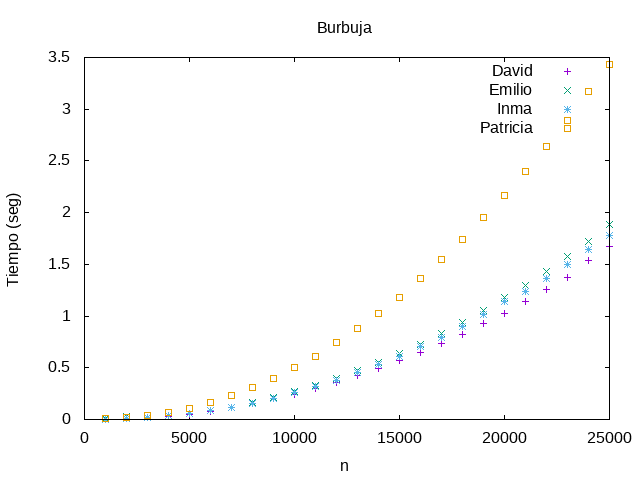
\includegraphics[width=90mm]{grupo/burbuja}}
	\subfigure[Inserción]{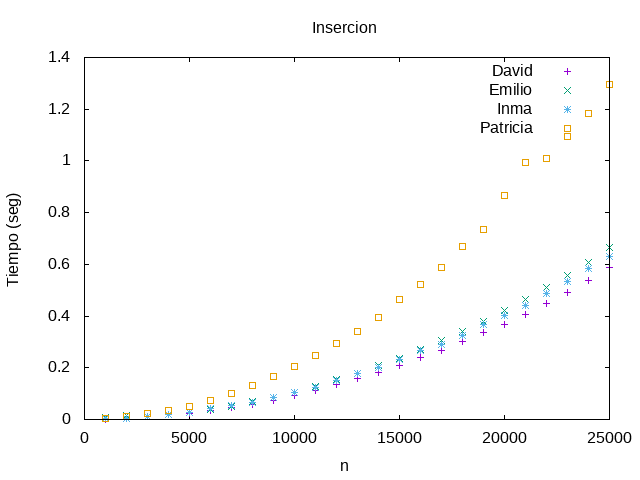
\includegraphics[width=90mm]{grupo/insercion}}
        \subfigure[Selección]{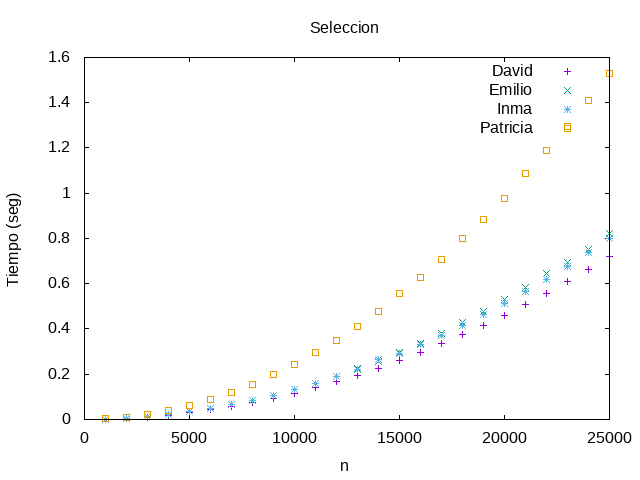
\includegraphics[width=90mm]{grupo/seleccion}}
\end{figure}
\subsection{Ordenación $O(n\log(n))$}

\begin{figure}[H]
	\centering
	\subfigure[Quicksort]{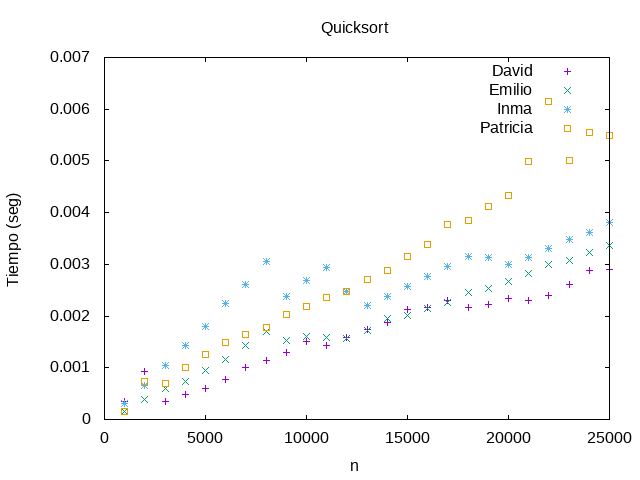
\includegraphics[width=90mm]{grupo/quicksort}}
	\subfigure[Mergesort]{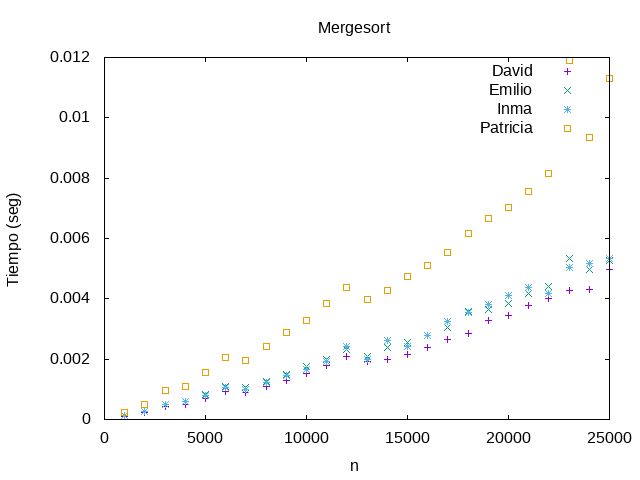
\includegraphics[width=90mm]{grupo/mergesort}}
        \subfigure[Heapsort]{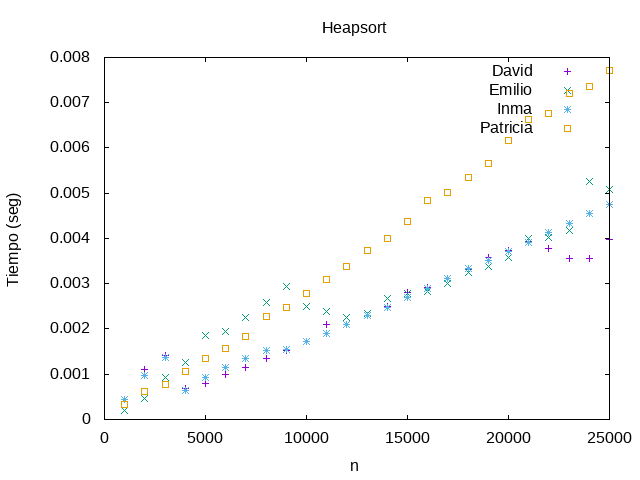
\includegraphics[width=90mm]{grupo/heapsort}}
      \end{figure}

\subsection{Floyd}

\begin{figure}[H]
	\centering
	\subfigure[Floyd]{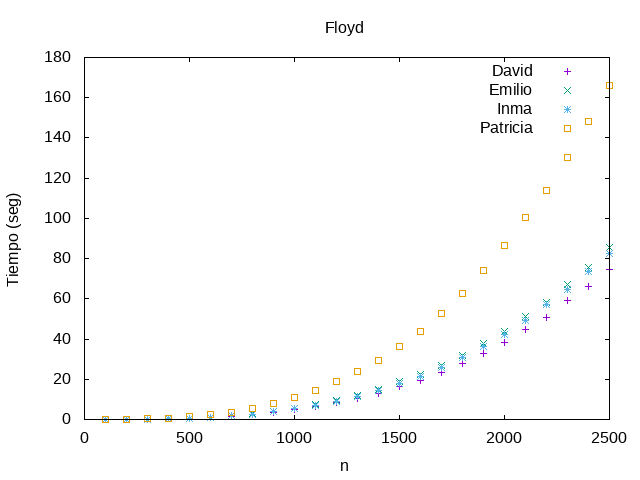
\includegraphics[width=90mm]{grupo/floyd}}
\end{figure}

\subsection{Hanoi}

\begin{figure}[H]
	\centering
	\subfigure[Hanoi]{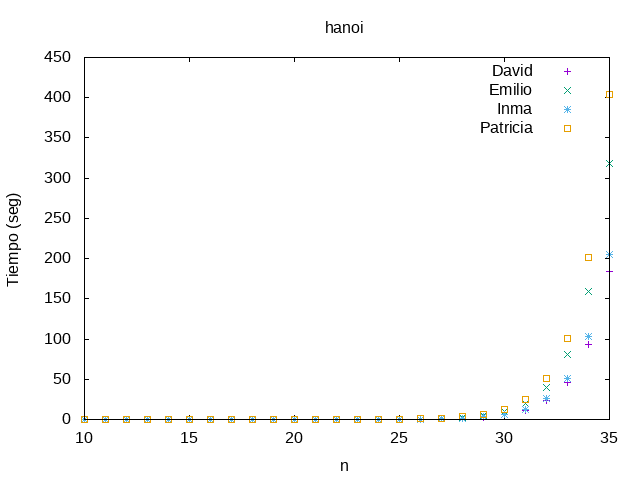
\includegraphics[width=90mm]{grupo/hanoi}}
\end{figure}

\begin{flushleft}
  Aunque los tiempos varíen debido a las características de nuestros
  ordenadores, puede apreciarse que el forma de las gráficas no
  cambia, podemos deducir que las características de un ordenador ni
  el sistema operativo no afectan al orden de eficiencia.
\end{flushleft}

\end{document}
